\documentclass{article}


\usepackage[italian]{}

\usepackage[letterpaper,top=2cm,bottom=2cm,left=3cm,right=3cm,marginparwidth=1.75cm]{geometry}

\usepackage{graphicx}
\usepackage{float}
\usepackage{longtable}

\title{ALBERI BINARI vs ALBERI ROSSO-NERI}
\author{Thomas Del Moro}

\begin{document}
\maketitle

\section{Introduzione}

In questo documento, come da titolo, confronteremo (dal punto di vista computazionale) Alberi Binari e Alberi Rosso-Neri. Faremo quindi un'analisi critica di alcuni algoritmi eseguibili su tali strutture dati, scelti in modo da evidenziarne differenze e somiglianze.

\subsection{Alberi Binari di Ricerca}

Gli alberi binari di ricerca (ABR) sono un particolare tipo di alberi di ricerca. La caratteristica che li contraddistingue è quella di avere al massimo due figli per ogni nodo ($x$). Tali figli sono chiamati figlio sinistro ($x.left$) e figlio destro ($x.right$). Ogni nodo è poi indicizzato attraverso una chiave ($x.key$).\\
La proprietà fondamentale degli ABR è la seguente:
\begin{itemize}
\item Se un nodo y è nel sottoalbero sinistro di un nodo x, allora $y.key < x.key$
\item Se un nodo y è nel sottoalbero destro di un nodo x, allora $y.key \geq x.key$
\end{itemize}
L'altezza dell'albero, che indichiamo con $h$, dipende quindi dall'ordine in cui vengono inserite le $n$ chiavi. Il caso peggiore, quello in cui le chiavi sono inserite in modo ordinato, corrisponde a un'altezza $h = n$. Il caso migliore invece è quello in cui le chiavi sono inserite in modo da bilanciare il più possibile l'albero e corrisponde quindi a un'altezza $h = lg(n)$

\subsection{Alberi Rosso-Neri}

Gli alberi rosso-neri (ARN) sono alberi binari di ricerca in cui ogni nodo $x$ eredita tutti gli attributi di un nodo di ABR ma ha un campo aggiuntivo: il colore ($x.color$), che può assumere valore "rosso" o "nero".\\
Tenendo conto delle proprietà degli ABR già elencate, vediamo quelle specifiche degli alberi rosso-neri:
\begin{itemize}
\item Ogni nodo è rosso o nero
\item La radice è nera
\item Ogni foglia è nera
\item Se un nodo è rosso, allora entrambi i suoi figli sono neri
\item Tutti i cammini da ogni nodo alle foglie contengono lo stesso numero di nodi neri
\end{itemize}
Grazie a tali proprietà, gli alberi rosso-neri risultano sempre approssimativamente bilanciati, ovvero la loro altezza rimane sempre logaritmica. In particolare, si può dimostrare che l'altezza di un albero rosso-nero con $n$ nodi è al massimo pari a $2lg(n+1)$

\subsection{ABR vs ARN - Risultati attesi}

Assumiamo di avere un numero di chiavi pari a $n$ e indichiamo l'altezza degli alberi con $h$
Le prestazioni degli algoritmi che analizzeremo, quali inserimento e ricerca, dipendono da $h$ e, in particolare, possiamo prevedere che abbiano un tempo di esecuzione asintotico $O(h)$.\\
Negli ABR non abbiamo un'indicazione a priori sull'altezza ma solo un caso migliore (albero bilanciato) per cui otterremo $h=lg(n)$, e un caso peggiore (chiavi in ordine crescente o decrescente), per cui risulterà $h=n$.
Negli ARN invece l'altezza è sempre logaritmica, dunque il tempo di esecuzione degli algoritmi sopra elencati sarà sempre $O(lg(n))$ (non c'è un caso migliore né uno peggiore).

\section{Esecuzione dei Test}

Ogni test è stato eseguito 100 volte attraverso un ciclo $for$, con un numero di chiavi $n$ che viene incrementato di 10000 chiavi a ogni iterazione del ciclo. Le chiavi vengono generate in maniera ordinata e salvate in una lista $keys$, la quale viene poi randomizzata attraverso la funzione shuffle().

\subsection{Inserimento}

Dopo aver generato le chiavi e averle ordinate in modo casuale, tali chiavi vengono inserite in sequenza all'interno di ognuno dei due alberi. Una volta inserite tutte le $n$ chiavi si calcola il tempo trascorso tra il primo inserimento e l'ultimo, attraverso il metodo $timer()$, così da avere una misura del tempo impiegato per eseguire tutti gli inserimenti.
Alla fine di ogni iterazione gli alberi vengono re-inizializzati, in modo da essere vuoti all'inizio del test successivo.\\
Contrariamente a quanto ci aspettavamo, ovvero una migliore efficienza dell'ARN, i risultati hanno evidenziato una netta similitudine nel tempo di inserimento dei due alberi, come è osservabile nel Grafico \ref{fig:mesh1} sotto riportato.
In realtà, quello che abbiamo ottenuto è un risultato plausibile: esso dipende dal fatto di aver ordinato le chiavi in modo casuale. In una tale condizione infatti, difficilmente l'ABR sarà tanto sbilanciato, dunque avrà un tempo di inserimento che assomiglia a quello logaritmico dell'albero rosso-nero.

\begin{figure}[h]
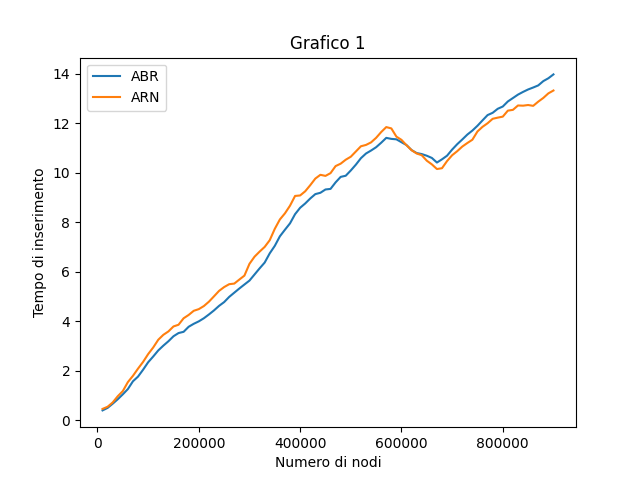
\includegraphics[height=10cm]{Figure_1.png}
\centering
\caption{Tempo (in secondi) impiegato per l'inserimento di $n$ nodi, al variare di $n$(numero di nodi)}
\label{fig:mesh1}
\end{figure}

\subsection{Ricerca}

A differenza del test precedente, siamo nella condizione in cui tutte le chiavi sono già state inserite. Si genera quindi un numero intero casuale e si ricerca tale chiave all'interno degli alberi, attraverso il metodo $treeSearch()$. Si è assunto che la chiave cercata sia sempre presente. Ovviamente per calcolare il tempo di esecuzione si utilizza la funzione $timer()$ come nel test precedente. Il test viene eseguito ad ogni iterazione del ciclo (ogni volta con un numero di chiavi maggiore).

\begin{figure}[h]
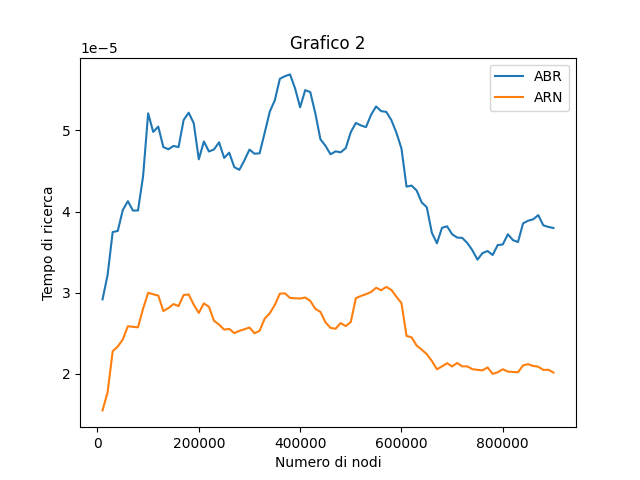
\includegraphics[height=10cm]{Figure_2.png}
\centering
\caption{Tempo (in secondi) impiegato per la ricerca di una chiave, al variare del numero di nodi}
\label{fig:mesh2}
\end{figure}

In accordo con le previsioni fatte in precedenza, nel Grafico \ref{fig:mesh2} possiamo osservare che l'ARN ha una maggiore efficienza (il tempo di esecuzione è all'incirca la metà), dovuta in particolare alla differenza di altezza tra i due alberi, che analizzeremo nella sezione seguente.\\
Già dall'algoritmo di ricerca possiamo quindi supporre che in molti casi sia vantaggioso utilizzare un ARN al posto di un semplice albero binario.

\subsection{Altezza}

L'ultimo test che abbiamo eseguito ha l'obiettivo di rendere esplicita la differenza di altezza tra ABR e ARN. Da essa infatti derivano i più evidenti vantaggi dell'uso degli alberi rosso-neri e, in particolare, i risultati dei test precedenti.
Il valore dell'altezza è stato calcolato con il metodo ricorsivo $treeHeight$, definito sia in ABR che in ARN.\\
I risultati, descritti nel Grafico \ref{fig:mesh3}, mostrano una netta differenza tra le due altezze. Sapevamo a priori che l'altezza $h$ di un albero rosso-nero è sempre $h\leq2lg(n+1)$, ma dall'esperimento possiamo evincere che in realtà l'ARN, generalmente, può fare molto meglio di così. A partire dai nostri dati, infatti, la sua altezza è quasi sempre proporzionale al $lg(n)$ (non solo a livello asintotico), mentre quella dell'ABR è, nella maggior parte dei casi, più del doppio.

\begin{figure}[H]
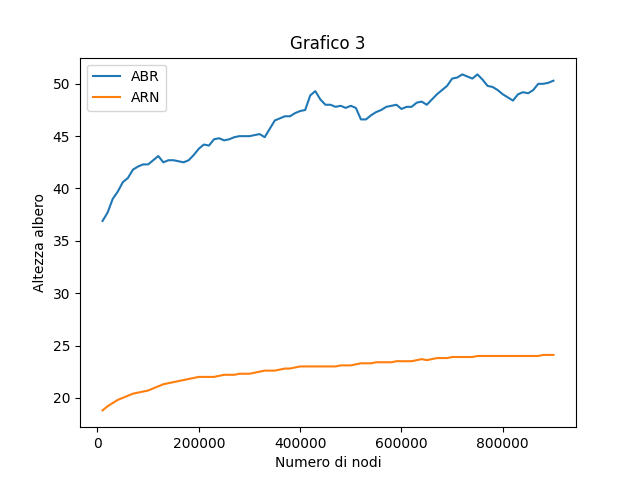
\includegraphics[height=9cm]{Figure_3.png}
\centering
\caption{Altezza degli alberi al variare del numero dei loro nodi}
\label{fig:mesh3}
\end{figure}

\subsection{Inserimento - verifica}
Poiché i tempi di inserimento sono risultati diversi da quelli che ci aspettavamo, abbiamo eseguito un ulteriore test sull'albero binario di ricerca, con meno valori rispetto ai test precedenti. Abbiamo infatti confrontato l'efficienza media (valori casuali) dell'inserimento nell'ABR con quella del caso peggiore (valori in input già ordinati).\\
Il Grafico \ref{fig:mesh4} mostra infatti una netta differenza tra i due casi, già inserendo pochi valori rispetto ai test precedenti. Questo può quindi giustificare, anche se solo in parte, i risultati precedenti.

\begin{figure}[H]
\centering
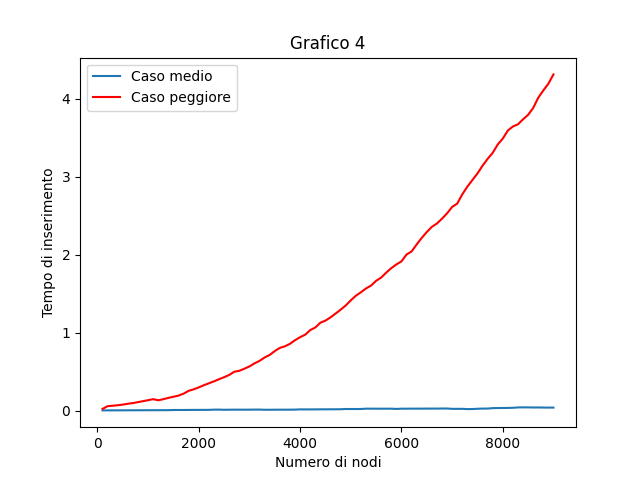
\includegraphics[height=9cm]{Figure_4.png}
\caption{Tempo di inserimento (in secondi) per numero di nodi}
\label{fig:mesh4}
\end{figure}


\section{Analisi complessiva degli esperimenti}

Gli esperimenti svolti hanno mostrato vantaggi e svantaggi di entrambe le strutture dati. Andando più nello specifico, analizziamo i risultati tratti dai vari test:
\begin{enumerate}
\item Per quanto riguarda l'inserimento, abbiamo dedotto che, se passiamo in ingresso chiavi in ordine casuale, il tempo di esecuzione è molto simile tra albero binario di ricerca e albero rosso-nero. L'ABR, infatti, molto probabilmente sarà abbastanza bilanciato e il suo algoritmo di inserimento avrà un costo asintotico simile a $O(lg(n))$. Inoltre, se ci concentriamo più sul costo esatto che su quello asintotico, dobbiamo considerare che l'ARN, ogni volta che viene inserito un nodo, deve chiamare la funzione $insertFixup()$, che a sua volta impiega $O(lg(n))$.
\item La ricerca invece mostra subito grandi differenze, già a partire da un basso numero di nodi, è evidente infatti che l'algoritmo impiega un tempo molto minore nell'albero rosso-nero. Dal grafico si può notare che nell'ARN ha un andamento logaritmico (in accordo con le previsioni), ma anche l'ABR, per quanto detto in precedenza, ha un tempo di ricerca con un andamento più simile a quello logaritmico che a quello lineare.
Nell'esperimento abbiamo assunto che tutte le chiavi cercate fossero presenti negli alberi, altrimenti il tempo di ricerca sarebbe stato strettamente legato all'altezza.
\item Infine il test sull'altezza ha mostrato quello che ci immaginavamo guardando i risultati degli altri test. Come è evidente nel Grafico \ref{fig:mesh3} l'altezza dell'ARN ha un andamento logaritmico. A conferma dei risultati ottenuti negli altri test, notiamo che anche l'ABR è abbastanza bilanciato, ma la sua altezza si allontana da quella dell'ARN all'aumentare del numero di nodi.

\end{enumerate}

\section{Conclusioni}
L'analisi critica dei test effettuati ha descritto quello che ci aspettavamo, ovvero una migliore efficienza degli alberi rosso-neri per quanto riguarda molti algoritmi. Allo stesso tempo possiamo concludere che se trattiamo un numero di elementi non eccessivo, possiamo comunque utilizzare gli alberi binari di ricerca e ottenere delle prestazioni simili a quelle degli ARN.

\section{Documentazione del codice}

\subsection{Contenuto e interazioni dei moduli}

Nel codice del file "main" sono stati importati i seguenti moduli:
\begin{itemize}
\item ABR : codice utilizzato per implementare gli alberi binari di ricerca e i corrispondenti algoritmi
\item ARN : codice utilizzato per implementare gli alberi rosso-neri e i corrispondenti algoritmi
\item random : codice per generare numeri casuali
\item timeit : codice per la definizione della funzione $timer()$
\item tabulate : codice per la generazione di tabelle che sono state esportate in questo documento
\item numpy : codice per scrittura matematica e per definire alcune funzioni usate, tra cui $convolve()$ e $arange()$
\item matplotlib : codice per generare i grafici sopra riportati
\end{itemize}

\subsection{Schema delle classi}

\begin{table}[h]
\centering
\begin{tabular}{|c|cc|}
\multicolumn{3}{c}{Schema delle Classi}\\
\hline
    Struttura dati &    Classe Nodo &   Classe Albero \\
\hline
               ABR &         Node   &             ABR \\
\hline
               ARN &         NodeRN &             ARN \\
\hline
\end{tabular}
\end{table}

\subsection{Metodi implementati}

ABR:
\begin{itemize}
\item init(self, key): costruisce un nodo a partire da una chiave
\item get(self): restituisce la chiave di un nodo
\item set(self, key): setta la chiave di un nodo al valore di key
\item init(self): costruttore dell'albero binario
\item setRoot(self, key): inizializza la radice dell'albero
\item treeSearch(self, key): chiama la funzione search() sulla radice dell'albero
\item search(self, currentNode, key): ricerca la chiave key nel sottoalbero con radice currentNode, se la ricerca ha successo restituisce il nodo trovato, altrimenti restituisce None
\item treeInorder(self): chiama la funzione inorder() sulla radice dell'albero
\item inorder(self, currentNode): esegue un attraversamento inorder sul sottoalbero con radice currentNode, ovvero stampa tutte le chiavi in ordine crescente
\item treeMinimum(self): chiama il metodo minimum() sulla radice dell'albero
\item minimum(self, currentNode): restituisce il nodo con chiave minima nel sottoalbero con radice currentNode
\item treeMaximum(self): chiama il metodo maximum() sulla radice dell'albero
\item maximum(self, currentNode): restituisce il nodo con chiave massima nel sottoalbero con radice currentNode
\item insert(self, key): inserisce un nodo con chiave key nell'albero
\item transplant(self, u, v): effettua un trapianto di sottoalberi (usato per la cancellazione)
\item delete(self, key): elimina il nodo con chiave key dall'albero
\item treeHeight(self): chiama la funzione height() sulla radice dell'albero
\item height(self, currentNode): restituisce l'altezza del sottoalbero con radice currentNode
\end{itemize}
ARN:
\begin{itemize}
\item init(self, key): costruisce un nodo con chiave key
\item init(self): costruisce un albero rosso-nero
\item setRoot(self, key): inizializza la radice dell'albero
\item leftRotate(self, x): effettua una rotazione a sinistra del sottoalbero con radice x
\item rightRotate(self, x): effettua una rotazione a destra del sottoalbero con radice x
\item insert(self, key): inserisce un nodo con chiave key nell'albero
\item insertFixup(self, z): effettua operazioni(cambi di colore e rotazioni) per garantire le proprietà dell'albero rosso-nero a seguito di un inserimento
\item treeInorder(self): chiama il metodo inorder() sulla radice dell'albero
\item inorder(self, currentNode): stampa tutte le chiavi del sottoalbero con radice currentNode, in ordine crescente
\item treePreorder(self): chiama il metodo preorder() sulla radice dell'albero
\item preorder(self, currentNode): stampa tutte le chiavi del sottoalbero con radice currentNode, in modo preorder
\item treePostorder(self): chiama il metodo postorder() sulla radice dell'albero
\item postorder(self, currentNode): stampa in modo postorder tutte le chiavi del sottoalbero con radice currentNode
\item treeHeight(self): chiama il metodo height() sulla radice dell'albero
\item height(self, currentNode): restituisce l'altezza del sottoalbero con radice currentNode
\item treeSearch(self, key): chiama il metodo search() sulla radice dell'albero
\item search(self, currentNode, key): ricerca un nodo con la chiave key nel sottoalbero di radice currentNode. Se lo trova, restituisce quel nodo, altrimenti ritorno valore nullo.
\end{itemize}
main:
\begin{itemize}
\item movingAverage(a): Prende in ingresso una lista e restituisce la media mobile dei suoi elementi
\item getAverages(i1, i2, s1, s2, h1, h2): per ogni lista passata in ingresso, ne calcola la media mobile con il metodo movingAverage()
\end{itemize}

\section{Hardware utilizzato}
Tutti i test sono stati effettuati su un computer portatile con le seguenti specifiche:\\
\\
CPU: Intel Core i7-8565U 1.80GHz 1.99GHz\\
RAM: 8GB DDR3\\
GPU: NVIDIA GeForceMX150\\
SO: Windows 10 Home

\newpage

\section{Tabelle}

\subsection{Inserimento}
{\renewcommand{\arraystretch}{0.9}}
{\centering}
\begin{longtable}{c|c|c}
\hline
\multicolumn{3}{c}{Test inserimento}\\
\hline
   Numero di nodi &   Tempo di inserimento ABR &   Tempo di inserimento ARN \\
\hline
            10000 &                      0.065 &                      0.096 \\
            20000 &                      0.132 &                      0.111 \\
            30000 &                      0.215 &                      0.299 \\
            40000 &                      0.154 &                      0.313 \\
            50000 &                      0.336 &                      0.359 \\
            60000 &                      0.419 &                      0.566 \\
            70000 &                      0.512 &                      0.597 \\
            80000 &                      0.678 &                      0.642 \\
            90000 &                      0.573 &                      0.698 \\
           100000 &                      0.941 &                      0.95  \\
           110000 &                      1.08  &                      0.964 \\
           120000 &                      1.814 &                      1.844 \\
           130000 &                      2.017 &                      2.812 \\
           140000 &                      2.147 &                      2.396 \\
           150000 &                      2.463 &                      3.986 \\
           160000 &                      3.562 &                      3.106 \\
           170000 &                      2.395 &                      3.497 \\
           180000 &                      3.46  &                      3.358 \\
           190000 &                      3.59  &                      3.852 \\
           200000 &                      3.266 &                      3.627 \\
           210000 &                      3.544 &                      4.094 \\
           220000 &                      3.741 &                      3.826 \\
           230000 &                      3.785 &                      4.181 \\
           240000 &                      4.166 &                      4.408 \\
           250000 &                      3.759 &                      4.679 \\
           260000 &                      4.065 &                      5.717 \\
           270000 &                      4.44  &                      4.846 \\
           280000 &                      4.651 &                      5.029 \\
           290000 &                      4.582 &                      4.528 \\
           300000 &                      4.522 &                      4.872 \\
           310000 &                      5.075 &                      5.859 \\
           320000 &                      5.378 &                      5.991 \\
           330000 &                      5.62  &                      6.379 \\
           340000 &                      5.681 &                      5.947 \\
           350000 &                      5.867 &                      5.84  \\
           360000 &                      5.762 &                      5.96  \\
           370000 &                      6.127 &                      6.476 \\
           380000 &                      6.261 &                      6.62  \\
           390000 &                      6.171 &                      9.294 \\
           400000 &                      6.991 &                      7.748 \\
           410000 &                      7.544 &                      7.913 \\
           420000 &                      7.716 &                      7.887 \\
           430000 &                      9.355 &                      9.098 \\
           440000 &                      8.705 &                     10.544 \\
           450000 &                      9.711 &                      9.615 \\
           460000 &                      8.42  &                      8.432 \\
           470000 &                      8.702 &                      9.564 \\
           480000 &                      9.976 &                     10.559 \\
           490000 &                      8.756 &                      9.496 \\
           500000 &                      8.73  &                      9.427 \\
           510000 &                      9.567 &                     10.392 \\
           520000 &                      9.474 &                     10.548 \\
           530000 &                      9.894 &                     10.619 \\
           540000 &                     10.038 &                     10.102 \\
           550000 &                      9.946 &                     10.732 \\
           560000 &                     11.062 &                     11.28  \\
           570000 &                     10.911 &                     10.537 \\
           580000 &                     10.439 &                     12.159 \\
           590000 &                     10.89  &                     10.706 \\
           600000 &                     11.073 &                     11.541 \\
           610000 &                     12.188 &                     12.5   \\
           620000 &                     11.357 &                     11.087 \\
           630000 &                     11.098 &                     11.651 \\
           640000 &                     11.378 &                     11.946 \\
           650000 &                     11.759 &                     13.063 \\
           660000 &                     13.022 &                     13.28  \\
           670000 &                     10.502 &                     10.008 \\
           680000 &                     10.263 &                      8.832 \\
           690000 &                      9.717 &                      9.411 \\
           700000 &                      9.921 &                      9.352 \\
           710000 &                     10.16  &                     10.498 \\
           720000 &                     10.16  &                      9.764 \\
           730000 &                     10.691 &                     10.953 \\
           740000 &                     10.707 &                      9.734 \\
           750000 &                     10.865 &                     11.575 \\
           760000 &                     11.165 &                     11.399 \\
           770000 &                     11.801 &                     10.34  \\
           780000 &                     11.732 &                     11.726 \\
           790000 &                     12.183 &                     11.757 \\
           800000 &                     12.09  &                     10.982 \\
           810000 &                     12.062 &                     12.369 \\
           820000 &                     12.148 &                     11.196 \\
           830000 &                     12.317 &                     12.29  \\
           840000 &                     12.637 &                     13.067 \\
           850000 &                     13.051 &                     13.452 \\
           860000 &                     13.302 &                     12.843 \\
           870000 &                     12.718 &                     12.137 \\
           880000 &                     13.354 &                     12.193 \\
           890000 &                     13.105 &                     12.168 \\
           900000 &                     14.131 &                     13.398 \\
           910000 &                     13.44  &                     12.69  \\
           920000 &                     13.537 &                     12.965 \\
           930000 &                     13.409 &                     12.208 \\
           940000 &                     13.623 &                     13.335 \\
           950000 &                     13.839 &                     13.111 \\
           960000 &                     14.154 &                     14.546 \\
           970000 &                     14.456 &                     13.637 \\
           980000 &                     14.507 &                     14.041 \\
           990000 &                     14.659 &                     13.319 \\
\hline
\caption{Tempi di inserimento per numero di nodi}
\end{longtable}

\newpage

\subsection{Ricerca}
{\centering}
{\renewcommand{\arraystretch}{0.9}}
\begin{longtable}{c|c|c}
\hline
\multicolumn{3}{c}{Test ricerca}\\
\hline
   Numero di nodi &   Tempo di ricerca ABR &   Tempo di ricerca ARN \\
\hline
            10000 &               1.98e-05 &               9.2e-06  \\
            20000 &               1.75e-05 &               7.8e-06  \\
            30000 &               3.75e-05 &               1.78e-05 \\
            40000 &               2.27e-05 &               1.52e-05 \\
            50000 &               3.24e-05 &               1.12e-05 \\
            60000 &               3.64e-05 &               1.66e-05 \\
            70000 &               3.39e-05 &               2.34e-05 \\
            80000 &               2.18e-05 &               1.54e-05 \\
            90000 &               2.02e-05 &               1.51e-05 \\
           100000 &               4.95e-05 &               2.31e-05 \\
           110000 &               4.99e-05 &               3.16e-05 \\
           120000 &               7.04e-05 &               5.83e-05 \\
           130000 &               3.89e-05 &               2.36e-05 \\
           140000 &               4.85e-05 &               2.4e-05  \\
           150000 &               4.33e-05 &               2.75e-05 \\
           160000 &               2.48e-05 &               1.58e-05 \\
           170000 &               3.4e-05  &               2.29e-05 \\
           180000 &               6.39e-05 &               3.83e-05 \\
           190000 &               9.79e-05 &               3.47e-05 \\
           200000 &               2.66e-05 &               2.13e-05 \\
           210000 &               5.64e-05 &               3e-05    \\
           220000 &               4.52e-05 &               3.92e-05 \\
           230000 &               3.62e-05 &               2.72e-05 \\
           240000 &               5.26e-05 &               2.9e-05  \\
           250000 &               4.18e-05 &               2.5e-05  \\
           260000 &               5.82e-05 &               2.95e-05 \\
           270000 &               4.31e-05 &               2.36e-05 \\
           280000 &               5.09e-05 &               2.56e-05 \\
           290000 &               5.34e-05 &               2.46e-05 \\
           300000 &               4.86e-05 &               3.31e-05 \\
           310000 &               4.4e-05  &               2.57e-05 \\
           320000 &               4.78e-05 &               2.21e-05 \\
           330000 &               4.5e-05  &               2.24e-05 \\
           340000 &               3.33e-05 &               2.28e-05 \\
           350000 &               4.83e-05 &               2.59e-05 \\
           360000 &               4.04e-05 &               2.43e-05 \\
           370000 &               3.97e-05 &               2.64e-05 \\
           380000 &               6.26e-05 &               2.75e-05 \\
           390000 &               6.67e-05 &               2.68e-05 \\
           400000 &               4.35e-05 &               2.6e-05  \\
           410000 &               4.45e-05 &               2.88e-05 \\
           420000 &               7.3e-05  &               3.7e-05  \\
           430000 &               7.1e-05  &               2.9e-05  \\
           440000 &               4.75e-05 &               3.31e-05 \\
           450000 &               7.48e-05 &               3.99e-05 \\
           460000 &               4.36e-05 &               2.46e-05 \\
           470000 &               4.19e-05 &               2.08e-05 \\
           480000 &               4.54e-05 &               2.7e-05  \\
           490000 &               4.33e-05 &               2.66e-05 \\
           500000 &               6.47e-05 &               2.72e-05 \\
           510000 &               4.21e-05 &               2.46e-05 \\
           520000 &               4.68e-05 &               2.72e-05 \\
           530000 &               3.91e-05 &               2.53e-05 \\
           540000 &               3.93e-05 &               2.03e-05 \\
           550000 &               6.44e-05 &               3.29e-05 \\
           560000 &               4.72e-05 &               2.36e-05 \\
           570000 &               4.07e-05 &               2.78e-05 \\
           580000 &               5.06e-05 &               2.32e-05 \\
           590000 &               6.3e-05  &               3.18e-05 \\
           600000 &               7.6e-05  &               5.65e-05 \\
           610000 &               3.91e-05 &               2.73e-05 \\
           620000 &               4.47e-05 &               2.94e-05 \\
           630000 &               5.43e-05 &               2.8e-05  \\
           640000 &               4.96e-05 &               2.55e-05 \\
           650000 &               5.86e-05 &               2.99e-05 \\
           660000 &               4.63e-05 &               2.77e-05 \\
           670000 &               3.06e-05 &               2.41e-05 \\
           680000 &               3.51e-05 &               1.48e-05 \\
           690000 &               4.34e-05 &               2.39e-05 \\
           700000 &               2.9e-05  &               1.6e-05  \\
           710000 &               4.04e-05 &               2.56e-05 \\
           720000 &               3.86e-05 &               1.92e-05 \\
           730000 &               3.96e-05 &               2.3e-05  \\
           740000 &               4.37e-05 &               1.99e-05 \\
           750000 &               2.71e-05 &               2.16e-05 \\
           760000 &               3.34e-05 &               1.74e-05 \\
           770000 &               4.96e-05 &               2.76e-05 \\
           780000 &               3.7e-05  &               1.88e-05 \\
           790000 &               3.36e-05 &               1.99e-05 \\
           800000 &               2.49e-05 &               2.03e-05 \\
           810000 &               4e-05    &               2.14e-05 \\
           820000 &               3.23e-05 &               1.92e-05 \\
           830000 &               3.06e-05 &               1.95e-05 \\
           840000 &               3.22e-05 &               1.91e-05 \\
           850000 &               3.52e-05 &               2.1e-05  \\
           860000 &               3.59e-05 &               2.1e-05  \\
           870000 &               4.47e-05 &               1.96e-05 \\
           880000 &               4.93e-05 &               2.08e-05 \\
           890000 &               3.43e-05 &               2.36e-05 \\
           900000 &               3.75e-05 &               1.75e-05 \\
           910000 &               3.28e-05 &               2.09e-05 \\
           920000 &               2.99e-05 &               1.88e-05 \\
           930000 &               5.36e-05 &               2.8e-05  \\
           940000 &               3.55e-05 &               2.06e-05 \\
           950000 &               3.69e-05 &               1.88e-05 \\
           960000 &               4.11e-05 &               2.01e-05 \\
           970000 &               3.21e-05 &               1.56e-05 \\
           980000 &               4.73e-05 &               2.1e-05  \\
           990000 &               3.3e-05  &               2.02e-05 \\
\hline
\caption{Tempi di ricerca per numero di nodi}
\end{longtable}

\newpage

\subsection{Altezza}
{\centering}
{\renewcommand{\arraystretch}{0.9}}
\begin{longtable}{c|c|c}
\hline
\multicolumn{3}{c}{Test altezza}\\
\hline
   Numero di nodi &   Altezza ABR &   Altezza ARN \\
\hline
            10000 &            33 &            16 \\
            20000 &            34 &            17 \\
            30000 &            34 &            18 \\
            40000 &            35 &            19 \\
            50000 &            39 &            19 \\
            60000 &            37 &            19 \\
            70000 &            39 &            20 \\
            80000 &            39 &            20 \\
            90000 &            39 &            20 \\
           100000 &            40 &            20 \\
           110000 &            41 &            20 \\
           120000 &            47 &            20 \\
           130000 &            41 &            21 \\
           140000 &            44 &            21 \\
           150000 &            43 &            21 \\
           160000 &            45 &            21 \\
           170000 &            42 &            21 \\
           180000 &            41 &            21 \\
           190000 &            39 &            21 \\
           200000 &            44 &            22 \\
           210000 &            45 &            22 \\
           220000 &            41 &            22 \\
           230000 &            43 &            22 \\
           240000 &            44 &            22 \\
           250000 &            42 &            22 \\
           260000 &            44 &            22 \\
           270000 &            44 &            22 \\
           280000 &            46 &            22 \\
           290000 &            45 &            22 \\
           300000 &            48 &            22 \\
           310000 &            44 &            22 \\
           320000 &            47 &            22 \\
           330000 &            44 &            23 \\
           340000 &            42 &            23 \\
           350000 &            43 &            22 \\
           360000 &            46 &            22 \\
           370000 &            45 &            23 \\
           380000 &            46 &            22 \\
           390000 &            45 &            22 \\
           400000 &            49 &            23 \\
           410000 &            45 &            23 \\
           420000 &            44 &            23 \\
           430000 &            52 &            23 \\
           440000 &            50 &            23 \\
           450000 &            45 &            23 \\
           460000 &            48 &            23 \\
           470000 &            45 &            23 \\
           480000 &            49 &            23 \\
           490000 &            47 &            23 \\
           500000 &            50 &            23 \\
           510000 &            59 &            23 \\
           520000 &            48 &            23 \\
           530000 &            44 &            23 \\
           540000 &            45 &            23 \\
           550000 &            45 &            23 \\
           560000 &            46 &            23 \\
           570000 &            46 &            24 \\
           580000 &            47 &            23 \\
           590000 &            49 &            23 \\
           600000 &            48 &            24 \\
           610000 &            48 &            24 \\
           620000 &            48 &            23 \\
           630000 &            48 &            23 \\
           640000 &            48 &            24 \\
           650000 &            47 &            23 \\
           660000 &            49 &            23 \\
           670000 &            47 &            24 \\
           680000 &            48 &            24 \\
           690000 &            45 &            23 \\
           700000 &            50 &            24 \\
           710000 &            48 &            24 \\
           720000 &            52 &            24 \\
           730000 &            49 &            24 \\
           740000 &            45 &            23 \\
           750000 &            52 &            24 \\
           760000 &            54 &            24 \\
           770000 &            51 &            24 \\
           780000 &            52 &            24 \\
           790000 &            52 &            24 \\
           800000 &            51 &            24 \\
           810000 &            51 &            24 \\
           820000 &            50 &            24 \\
           830000 &            47 &            24 \\
           840000 &            49 &            24 \\
           850000 &            47 &            24 \\
           860000 &            48 &            24 \\
           870000 &            50 &            24 \\
           880000 &            49 &            24 \\
           890000 &            48 &            24 \\
           900000 &            48 &            24 \\
           910000 &            48 &            24 \\
           920000 &            56 &            24 \\
           930000 &            49 &            24 \\
           940000 &            48 &            24 \\
           950000 &            50 &            24 \\
           960000 &            54 &            24 \\
           970000 &            50 &            25 \\
           980000 &            50 &            24 \\
           990000 &            50 &            24 \\
\hline
\caption{Altezza degli alberi per numero di nodi}
\end{longtable}

\newpage

\subsection{Inserimento ABR}
{\centering}
{\renewcommand{\arraystretch}{0.9}}
\begin{longtable}{c|c|c}
\hline
\multicolumn{3}{c}{Test inserimento ABR}\\
\hline
   Numero di nodi &   Caso medio &   Caso peggiore \\
\hline
              100 &        0     &           0.001 \\
              200 &        0     &           0.003 \\
              300 &        0.001 &           0.005 \\
              400 &        0.001 &           0.009 \\
              500 &        0.002 &           0.017 \\
              600 &        0.002 &           0.024 \\
              700 &        0.002 &           0.033 \\
              800 &        0.003 &           0.041 \\
              900 &        0.001 &           0.033 \\
             1000 &        0.003 &           0.042 \\
             1100 &        0.003 &           0.351 \\
             1200 &        0.003 &           0.059 \\
             1300 &        0.002 &           0.068 \\
             1400 &        0.004 &           0.088 \\
             1500 &        0.006 &           0.128 \\
             1600 &        0.004 &           0.112 \\
             1700 &        0.003 &           0.157 \\
             1800 &        0.006 &           0.16  \\
             1900 &        0.004 &           0.161 \\
             2000 &        0.004 &           0.173 \\
             2100 &        0.005 &           0.206 \\
             2200 &        0.005 &           0.201 \\
             2300 &        0.005 &           0.235 \\
             2400 &        0.026 &           0.235 \\
             2500 &        0.006 &           0.277 \\
             2600 &        0.005 &           0.362 \\
             2700 &        0.006 &           0.516 \\
             2800 &        0.012 &           0.356 \\
             2900 &        0.006 &           0.409 \\
             3000 &        0.006 &           0.449 \\
             3100 &        0.007 &           0.455 \\
             3200 &        0.032 &           0.454 \\
             3300 &        0.008 &           0.509 \\
             3400 &        0.007 &           0.486 \\
             3500 &        0.014 &           0.568 \\
             3600 &        0.01  &           0.772 \\
             3700 &        0.008 &           0.638 \\
             3800 &        0.008 &           0.623 \\
             3900 &        0.008 &           0.703 \\
             4000 &        0.016 &           0.842 \\
             4100 &        0.009 &           0.778 \\
             4200 &        0.009 &           0.886 \\
             4300 &        0.009 &           0.837 \\
             4400 &        0.014 &           0.982 \\
             4500 &        0.016 &           0.973 \\
             4600 &        0.01  &           0.979 \\
             4700 &        0.011 &           0.957 \\
             4800 &        0.012 &           1.088 \\
             4900 &        0.04  &           1.083 \\
             5000 &        0.012 &           1.166 \\
             5100 &        0.011 &           1.368 \\
             5200 &        0.011 &           1.216 \\
             5300 &        0.015 &           1.455 \\
             5400 &        0.015 &           1.246 \\
             5500 &        0.019 &           1.397 \\
             5600 &        0.012 &           1.463 \\
             5700 &        0.016 &           1.452 \\
             5800 &        0.047 &           1.628 \\
             5900 &        0.033 &           1.739 \\
             6000 &        0.014 &           1.758 \\
             6100 &        0.014 &           1.814 \\
             6200 &        0.052 &           1.702 \\
             6300 &        0.014 &           1.829 \\
             6400 &        0.014 &           1.856 \\
             6500 &        0.016 &           1.817 \\
             6600 &        0.015 &           2.098 \\
             6700 &        0.016 &           2.026 \\
             6800 &        0.015 &           2.097 \\
             6900 &        0.063 &           2.136 \\
             7000 &        0.016 &           2.629 \\
             7100 &        0.019 &           2.214 \\
             7200 &        0.05  &           2.596 \\
             7300 &        0.018 &           2.674 \\
             7400 &        0.017 &           2.605 \\
             7500 &        0.017 &           2.482 \\
             7600 &        0.017 &           2.527 \\
             7700 &        0.022 &           2.644 \\
             7800 &        0.019 &           2.782 \\
             7900 &        0.018 &           2.961 \\
             8000 &        0.018 &           3.053 \\
             8100 &        0.018 &           3.399 \\
             8200 &        0.019 &           3.582 \\
             8300 &        0.024 &           3.527 \\
             8400 &        0.052 &           3.448 \\
             8500 &        0.04  &           3.476 \\
             8600 &        0.021 &           3.401 \\
             8700 &        0.075 &           3.42  \\
             8800 &        0.034 &           3.849 \\
             8900 &        0.026 &           3.723 \\
             9000 &        0.022 &           4.095 \\
             9100 &        0.038 &           3.908 \\
             9200 &        0.063 &           3.866 \\
             9300 &        0.031 &           4.167 \\
             9400 &        0.053 &           4.023 \\
             9500 &        0.024 &           4.354 \\
             9600 &        0.027 &           4.719 \\
             9700 &        0.062 &           4.352 \\
             9800 &        0.03  &           4.713 \\
             9900 &        0.024 &           4.915 \\
\hline
\caption{Tempo di inserimento per numero di nodi}
\end{longtable}

\end{document}
